\documentclass[twoside]{book}

% Packages required by doxygen
\usepackage{fixltx2e}
\usepackage{calc}
\usepackage{doxygen}
\usepackage[export]{adjustbox} % also loads graphicx
\usepackage{graphicx}
\usepackage[utf8]{inputenc}
\usepackage{makeidx}
\usepackage{multicol}
\usepackage{multirow}
\PassOptionsToPackage{warn}{textcomp}
\usepackage{textcomp}
\usepackage[nointegrals]{wasysym}
\usepackage[table]{xcolor}

% NLS support packages
\usepackage[T2A]{fontenc}
\usepackage[russian]{babel}

% Font selection
\usepackage[T1]{fontenc}
\usepackage[scaled=.90]{helvet}
\usepackage{courier}
\usepackage{amssymb}
\usepackage{sectsty}
\renewcommand{\familydefault}{\sfdefault}
\allsectionsfont{%
  \fontseries{bc}\selectfont%
  \color{darkgray}%
}
\renewcommand{\DoxyLabelFont}{%
  \fontseries{bc}\selectfont%
  \color{darkgray}%
}
\newcommand{\+}{\discretionary{\mbox{\scriptsize$\hookleftarrow$}}{}{}}

% Page & text layout
\usepackage{geometry}
\geometry{%
  a4paper,%
  top=2.5cm,%
  bottom=2.5cm,%
  left=2.5cm,%
  right=2.5cm%
}
\tolerance=750
\hfuzz=15pt
\hbadness=750
\setlength{\emergencystretch}{15pt}
\setlength{\parindent}{0cm}
\setlength{\parskip}{3ex plus 2ex minus 2ex}
\makeatletter
\renewcommand{\paragraph}{%
  \@startsection{paragraph}{4}{0ex}{-1.0ex}{1.0ex}{%
    \normalfont\normalsize\bfseries\SS@parafont%
  }%
}
\renewcommand{\subparagraph}{%
  \@startsection{subparagraph}{5}{0ex}{-1.0ex}{1.0ex}{%
    \normalfont\normalsize\bfseries\SS@subparafont%
  }%
}
\makeatother

% Headers & footers
\usepackage{fancyhdr}
\pagestyle{fancyplain}
\fancyhead[LE]{\fancyplain{}{\bfseries\thepage}}
\fancyhead[CE]{\fancyplain{}{}}
\fancyhead[RE]{\fancyplain{}{\bfseries\leftmark}}
\fancyhead[LO]{\fancyplain{}{\bfseries\rightmark}}
\fancyhead[CO]{\fancyplain{}{}}
\fancyhead[RO]{\fancyplain{}{\bfseries\thepage}}
\fancyfoot[LE]{\fancyplain{}{}}
\fancyfoot[CE]{\fancyplain{}{}}
\fancyfoot[RE]{\fancyplain{}{\bfseries\scriptsize Создано системой Doxygen }}
\fancyfoot[LO]{\fancyplain{}{\bfseries\scriptsize Создано системой Doxygen }}
\fancyfoot[CO]{\fancyplain{}{}}
\fancyfoot[RO]{\fancyplain{}{}}
\renewcommand{\footrulewidth}{0.4pt}
\renewcommand{\chaptermark}[1]{%
  \markboth{#1}{}%
}
\renewcommand{\sectionmark}[1]{%
  \markright{\thesection\ #1}%
}

% Indices & bibliography
\usepackage{natbib}
\usepackage[titles]{tocloft}
\setcounter{tocdepth}{3}
\setcounter{secnumdepth}{5}
\makeindex

% Hyperlinks (required, but should be loaded last)
\usepackage{ifpdf}
\ifpdf
  \usepackage[pdftex,pagebackref=true]{hyperref}
\else
  \usepackage[ps2pdf,pagebackref=true]{hyperref}
\fi
\hypersetup{%
  colorlinks=true,%
  linkcolor=blue,%
  citecolor=blue,%
  unicode%
}

% Custom commands
\newcommand{\clearemptydoublepage}{%
  \newpage{\pagestyle{empty}\cleardoublepage}%
}

\usepackage{caption}
\captionsetup{labelsep=space,justification=centering,font={bf},singlelinecheck=off,skip=4pt,position=top}

%===== C O N T E N T S =====

\begin{document}

% Titlepage & ToC
\hypersetup{pageanchor=false,
             bookmarksnumbered=true,
             pdfencoding=unicode
            }
\pagenumbering{roman}
\begin{titlepage}
\vspace*{7cm}
\begin{center}%
{\Large B\+D\+D-\/education \\[1ex]\large 0.\+2 }\\
\vspace*{1cm}
{\large Создано системой Doxygen 1.8.11}\\
\end{center}
\end{titlepage}
\clearemptydoublepage
\tableofcontents
\clearemptydoublepage
\pagenumbering{arabic}
\hypersetup{pageanchor=true}

%--- Begin generated contents ---
\chapter{Список задач}
\label{todo}
\hypertarget{todo}{}

\begin{DoxyRefList}
\item[\label{todo__todo000001}%
\hypertarget{todo__todo000001}{}%
Класс \hyperlink{class_graph}{Graph} ]Добавить функцию построения несокращенной БДР 
\end{DoxyRefList}
\chapter{Иерархический список классов}
\section{Иерархия классов}
Иерархия классов.\begin{DoxyCompactList}
\item \contentsline{section}{Function}{\pageref{class_function}}{}
\item \contentsline{section}{Graph}{\pageref{class_graph}}{}
\item \contentsline{section}{Node}{\pageref{class_node}}{}
\item Q\+Main\+Window\begin{DoxyCompactList}
\item \contentsline{section}{Main\+Window}{\pageref{class_main_window}}{}
\end{DoxyCompactList}
\end{DoxyCompactList}

\chapter{Алфавитный указатель классов}
\section{Классы}
Классы с их кратким описанием.\begin{DoxyCompactList}
\item\contentsline{section}{\hyperlink{class_function}{Function} \\*Логическая функция и вектор ее значений }{\pageref{class_function}}{}
\item\contentsline{section}{\hyperlink{class_graph}{Graph} \\*Сокращенная упорядоченная бинарная диаграмма решений, представленная в виде графа }{\pageref{class_graph}}{}
\item\contentsline{section}{\hyperlink{class_main_window}{Main\+Window} }{\pageref{class_main_window}}{}
\item\contentsline{section}{\hyperlink{class_node}{Node} \\*Узел БДР }{\pageref{class_node}}{}
\end{DoxyCompactList}

\chapter{Классы}
\hypertarget{class_function}{}\section{Класс Function}
\label{class_function}\index{Function@{Function}}


Логическая функция и вектор ее значений  




{\ttfamily \#include $<$function.\+h$>$}

\subsection*{Открытые члены}
\begin{DoxyCompactItemize}
\item 
void \hyperlink{class_function_a6442bf1b8534028339904204a5b56949}{calculate\+Values} ()
\begin{DoxyCompactList}\small\item\em Вычисление вектора значений логической функции \end{DoxyCompactList}\item 
void \hyperlink{class_function_a027f157bb949b9598b08db6596c3e291}{set\+Formula} (Q\+String \+\_\+formula)
\begin{DoxyCompactList}\small\item\em Изменить запись функции \end{DoxyCompactList}\item 
Q\+String \hyperlink{class_function_af9036d1aabffcd855c0d3e4981ec7f0a}{get\+Formula} ()
\item 
Q\+Char \hyperlink{class_function_a87ff969fd64a5dcdacdca843a3dc13fb}{get\+Number\+Of\+Variables} ()
\item 
Q\+String \hyperlink{class_function_a23aa5c7ecc12e85f6cf7d175394d3a64}{get\+Values} ()
\begin{DoxyCompactList}\small\item\em Вывод вектора значений \end{DoxyCompactList}\end{DoxyCompactItemize}


\subsection{Подробное описание}
Логическая функция и вектор ее значений 

\begin{DoxyWarning}{Предупреждения}
Вектор значений функции представлен 32-\/битным машинным словом. Из этого следует, что функция не может иметь более пяти переменных. 
\end{DoxyWarning}


\subsection{Методы}
\index{Function@{Function}!calculate\+Values@{calculate\+Values}}
\index{calculate\+Values@{calculate\+Values}!Function@{Function}}
\subsubsection[{\texorpdfstring{calculate\+Values()}{calculateValues()}}]{\setlength{\rightskip}{0pt plus 5cm}void Function\+::calculate\+Values (
\begin{DoxyParamCaption}
{}
\end{DoxyParamCaption}
)}\hypertarget{class_function_a6442bf1b8534028339904204a5b56949}{}\label{class_function_a6442bf1b8534028339904204a5b56949}


Вычисление вектора значений логической функции 

Находится число переменных логической функции, вычисляются значения функции при каждом наборе значений переменных. \index{Function@{Function}!get\+Formula@{get\+Formula}}
\index{get\+Formula@{get\+Formula}!Function@{Function}}
\subsubsection[{\texorpdfstring{get\+Formula()}{getFormula()}}]{\setlength{\rightskip}{0pt plus 5cm}Q\+String Function\+::get\+Formula (
\begin{DoxyParamCaption}
{}
\end{DoxyParamCaption}
)}\hypertarget{class_function_af9036d1aabffcd855c0d3e4981ec7f0a}{}\label{class_function_af9036d1aabffcd855c0d3e4981ec7f0a}
\begin{DoxyReturn}{Возвращает}
Строку, содержащую запись функции 
\end{DoxyReturn}
\index{Function@{Function}!get\+Number\+Of\+Variables@{get\+Number\+Of\+Variables}}
\index{get\+Number\+Of\+Variables@{get\+Number\+Of\+Variables}!Function@{Function}}
\subsubsection[{\texorpdfstring{get\+Number\+Of\+Variables()}{getNumberOfVariables()}}]{\setlength{\rightskip}{0pt plus 5cm}Q\+Char Function\+::get\+Number\+Of\+Variables (
\begin{DoxyParamCaption}
{}
\end{DoxyParamCaption}
)}\hypertarget{class_function_a87ff969fd64a5dcdacdca843a3dc13fb}{}\label{class_function_a87ff969fd64a5dcdacdca843a3dc13fb}
\begin{DoxyReturn}{Возвращает}
Количество переменных функции 
\end{DoxyReturn}
\index{Function@{Function}!get\+Values@{get\+Values}}
\index{get\+Values@{get\+Values}!Function@{Function}}
\subsubsection[{\texorpdfstring{get\+Values()}{getValues()}}]{\setlength{\rightskip}{0pt plus 5cm}Q\+String Function\+::get\+Values (
\begin{DoxyParamCaption}
{}
\end{DoxyParamCaption}
)}\hypertarget{class_function_a23aa5c7ecc12e85f6cf7d175394d3a64}{}\label{class_function_a23aa5c7ecc12e85f6cf7d175394d3a64}


Вывод вектора значений 

\begin{DoxyReturn}{Возвращает}
Строковую запись вектора значений 
\end{DoxyReturn}
\index{Function@{Function}!set\+Formula@{set\+Formula}}
\index{set\+Formula@{set\+Formula}!Function@{Function}}
\subsubsection[{\texorpdfstring{set\+Formula(\+Q\+String \+\_\+formula)}{setFormula(QString _formula)}}]{\setlength{\rightskip}{0pt plus 5cm}void Function\+::set\+Formula (
\begin{DoxyParamCaption}
\item[{Q\+String}]{\+\_\+formula}
\end{DoxyParamCaption}
)}\hypertarget{class_function_a027f157bb949b9598b08db6596c3e291}{}\label{class_function_a027f157bb949b9598b08db6596c3e291}


Изменить запись функции 


\begin{DoxyParams}{Аргументы}
{\em \+\_\+formula} & \\
\hline
\end{DoxyParams}


Объявления и описания членов классов находятся в файлах\+:\begin{DoxyCompactItemize}
\item 
C\+:/\+Users/\+Alexander/\+Documents/\+B\+D\+D\+\_\+education/function.\+h\item 
C\+:/\+Users/\+Alexander/\+Documents/\+B\+D\+D\+\_\+education/function.\+cpp\end{DoxyCompactItemize}

\hypertarget{class_graph}{}\section{Класс Graph}
\label{class_graph}\index{Graph@{Graph}}


Сокращенная упорядоченная бинарная диаграмма решений, представленная в виде графа  




{\ttfamily \#include $<$graph.\+h$>$}

\subsection*{Открытые члены}
\begin{DoxyCompactItemize}
\item 
\hyperlink{class_graph_ae4c72b8ac4d693c49800a4c7e273654f}{Graph} ()\hypertarget{class_graph_ae4c72b8ac4d693c49800a4c7e273654f}{}\label{class_graph_ae4c72b8ac4d693c49800a4c7e273654f}

\begin{DoxyCompactList}\small\item\em Инициализация ключевых узлов БДР (0-\/терминальный узел, 1-\/терминальный узел, корень диаграммы) \end{DoxyCompactList}\item 
\hyperlink{class_graph_a902c5b3eacb66d60752525ab23297a95}{$\sim$\+Graph} ()\hypertarget{class_graph_a902c5b3eacb66d60752525ab23297a95}{}\label{class_graph_a902c5b3eacb66d60752525ab23297a95}

\begin{DoxyCompactList}\small\item\em Удаление диаграммы \end{DoxyCompactList}\item 
void \hyperlink{class_graph_a2a51a5b554d072c8fcfa934cabf08779}{build\+Bdd} (int values, int variables, \hyperlink{class_node}{Node} $\ast$node, int number=1)
\begin{DoxyCompactList}\small\item\em Построение БДР булевой функции по ее вектору значений \end{DoxyCompactList}\item 
\hyperlink{class_node}{Node} $\ast$ \hyperlink{class_graph_aa706260b27686591003a41c2b8c42644}{get\+Root} ()\hypertarget{class_graph_aa706260b27686591003a41c2b8c42644}{}\label{class_graph_aa706260b27686591003a41c2b8c42644}

\begin{DoxyCompactList}\small\item\em Возвращает указатель на корень диаграммы \end{DoxyCompactList}\end{DoxyCompactItemize}


\subsection{Подробное описание}
Сокращенная упорядоченная бинарная диаграмма решений, представленная в виде графа 

\begin{DoxyAuthor}{Автор}
Александр Митюнин 
\end{DoxyAuthor}
\begin{DoxyRefDesc}{Необходимо сделать}
\item[\hyperlink{todo__todo000001}{Необходимо сделать}]Добавить функцию построения несокращенной БДР \end{DoxyRefDesc}


\subsection{Методы}
\index{Graph@{Graph}!build\+Bdd@{build\+Bdd}}
\index{build\+Bdd@{build\+Bdd}!Graph@{Graph}}
\subsubsection[{\texorpdfstring{build\+Bdd(int values, int variables, Node $\ast$node, int number=1)}{buildBdd(int values, int variables, Node *node, int number=1)}}]{\setlength{\rightskip}{0pt plus 5cm}void Graph\+::build\+Bdd (
\begin{DoxyParamCaption}
\item[{int}]{values, }
\item[{int}]{variables, }
\item[{{\bf Node} $\ast$}]{node, }
\item[{int}]{number = {\ttfamily 1}}
\end{DoxyParamCaption}
)}\hypertarget{class_graph_a2a51a5b554d072c8fcfa934cabf08779}{}\label{class_graph_a2a51a5b554d072c8fcfa934cabf08779}


Построение БДР булевой функции по ее вектору значений 


\begin{DoxyParams}{Аргументы}
{\em values} & Вектор значений функции в форме машинного слова \\
\hline
{\em variables} & Число переменных \\
\hline
{\em node} & Корень диаграммы \\
\hline
{\em number} & Индекс текущей переменной \\
\hline
\end{DoxyParams}


Объявления и описания членов классов находятся в файлах\+:\begin{DoxyCompactItemize}
\item 
C\+:/\+Users/\+Alexander/\+Documents/\+B\+D\+D\+\_\+education/graph.\+h\item 
C\+:/\+Users/\+Alexander/\+Documents/\+B\+D\+D\+\_\+education/graph.\+cpp\end{DoxyCompactItemize}

\hypertarget{class_main_window}{}\section{Класс Main\+Window}
\label{class_main_window}\index{Main\+Window@{Main\+Window}}
Граф наследования\+:Main\+Window\+:\begin{figure}[H]
\begin{center}
\leavevmode
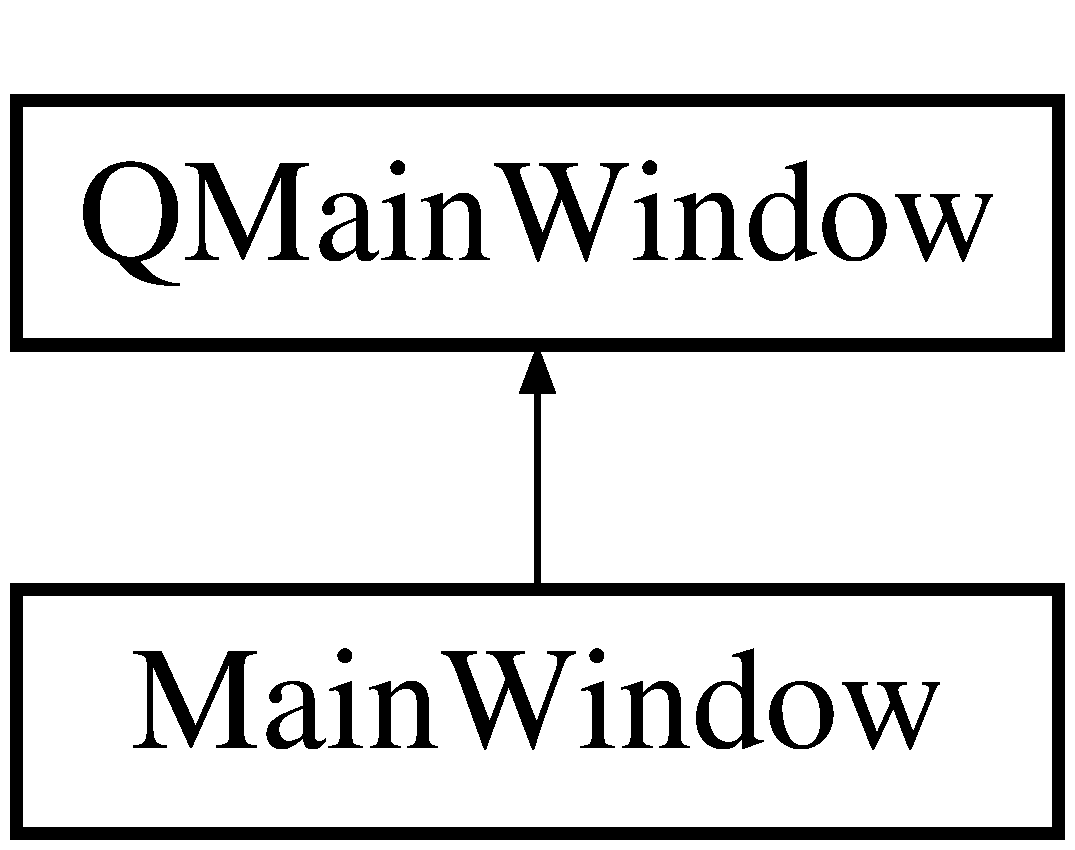
\includegraphics[height=2.000000cm]{class_main_window}
\end{center}
\end{figure}
\subsection*{Открытые члены}
\begin{DoxyCompactItemize}
\item 
{\bfseries Main\+Window} (Q\+Widget $\ast$parent=0)\hypertarget{class_main_window_a8b244be8b7b7db1b08de2a2acb9409db}{}\label{class_main_window_a8b244be8b7b7db1b08de2a2acb9409db}

\end{DoxyCompactItemize}


Объявления и описания членов классов находятся в файлах\+:\begin{DoxyCompactItemize}
\item 
C\+:/\+Users/\+Alexander/\+Documents/\+B\+D\+D\+\_\+education/mainwindow.\+h\item 
C\+:/\+Users/\+Alexander/\+Documents/\+B\+D\+D\+\_\+education/mainwindow.\+cpp\end{DoxyCompactItemize}

\hypertarget{class_node}{}\section{Класс Node}
\label{class_node}\index{Node@{Node}}


Узел БДР  




{\ttfamily \#include $<$node.\+h$>$}

\subsection*{Открытые члены}
\begin{DoxyCompactItemize}
\item 
\hyperlink{class_node_ad7a34779cad45d997bfd6d3d8043c75f}{Node} ()\hypertarget{class_node_ad7a34779cad45d997bfd6d3d8043c75f}{}\label{class_node_ad7a34779cad45d997bfd6d3d8043c75f}

\begin{DoxyCompactList}\small\item\em Создает узел без пометки и без связей \end{DoxyCompactList}\item 
\hyperlink{class_node_a184f393e8d61eea5e10fd6794cbd9c8d}{Node} (Q\+String \+\_\+data, \hyperlink{class_node}{Node} $\ast$low, \hyperlink{class_node}{Node} $\ast$high)
\begin{DoxyCompactList}\small\item\em Создает узел с заданными пометкой и связями \end{DoxyCompactList}\item 
Q\+String \hyperlink{class_node_ab3be314a19ff6049d0ab528ef3122139}{get\+Data} ()\hypertarget{class_node_ab3be314a19ff6049d0ab528ef3122139}{}\label{class_node_ab3be314a19ff6049d0ab528ef3122139}

\begin{DoxyCompactList}\small\item\em Возвращает строку, содержащую пометку узла \end{DoxyCompactList}\item 
void \hyperlink{class_node_a4ec7f6f38e67963aed6759a782db25a1}{set\+Data} (Q\+String \+\_\+data)\hypertarget{class_node_a4ec7f6f38e67963aed6759a782db25a1}{}\label{class_node_a4ec7f6f38e67963aed6759a782db25a1}

\begin{DoxyCompactList}\small\item\em Изменяет пометку узла на заданную \end{DoxyCompactList}\item 
void \hyperlink{class_node_afd304ef1773b4ee5e75e826c4b7b57b0}{set\+Low\+Connection} (\hyperlink{class_node}{Node} $\ast$node)\hypertarget{class_node_afd304ef1773b4ee5e75e826c4b7b57b0}{}\label{class_node_afd304ef1773b4ee5e75e826c4b7b57b0}

\begin{DoxyCompactList}\small\item\em Задает адрес младшего потомка \end{DoxyCompactList}\item 
void \hyperlink{class_node_ab8a35e02d194a5f378120db368a22ded}{set\+Low\+Connection} (Q\+String \+\_\+data)\hypertarget{class_node_ab8a35e02d194a5f378120db368a22ded}{}\label{class_node_ab8a35e02d194a5f378120db368a22ded}

\begin{DoxyCompactList}\small\item\em Создает узел с заданной пометкой без связей и назначает его младшим потомком \end{DoxyCompactList}\item 
void \hyperlink{class_node_a77ee961e6ac046ecc4f52e2cea94ad19}{set\+High\+Connection} (\hyperlink{class_node}{Node} $\ast$node)\hypertarget{class_node_a77ee961e6ac046ecc4f52e2cea94ad19}{}\label{class_node_a77ee961e6ac046ecc4f52e2cea94ad19}

\begin{DoxyCompactList}\small\item\em Задает адрес старшего потомка \end{DoxyCompactList}\item 
void \hyperlink{class_node_a14d42baec35f7dcbe6273fb4e91132e3}{set\+High\+Connection} (Q\+String \+\_\+data)\hypertarget{class_node_a14d42baec35f7dcbe6273fb4e91132e3}{}\label{class_node_a14d42baec35f7dcbe6273fb4e91132e3}

\begin{DoxyCompactList}\small\item\em Создает узел с заданной пометкой без связей и назначает его старшим потомком \end{DoxyCompactList}\item 
\hyperlink{class_node}{Node} $\ast$ \hyperlink{class_node_abf9a87b58ca04ff3c730e2097eee6f19}{get\+High} ()\hypertarget{class_node_abf9a87b58ca04ff3c730e2097eee6f19}{}\label{class_node_abf9a87b58ca04ff3c730e2097eee6f19}

\begin{DoxyCompactList}\small\item\em Возвращает указатель на старшего потомка \end{DoxyCompactList}\item 
\hyperlink{class_node}{Node} $\ast$ \hyperlink{class_node_adf1eae3c27b3b6fb038f2a677743e4c3}{get\+Low} ()\hypertarget{class_node_adf1eae3c27b3b6fb038f2a677743e4c3}{}\label{class_node_adf1eae3c27b3b6fb038f2a677743e4c3}

\begin{DoxyCompactList}\small\item\em Возвращает указатель на младшего потомка \end{DoxyCompactList}\item 
void \hyperlink{class_node_afaad8bb158fae2f283ef8d034c7b1723}{delink} (\hyperlink{class_node}{Node} $\ast$address)
\begin{DoxyCompactList}\small\item\em Удаление связей с заданным узлом \end{DoxyCompactList}\end{DoxyCompactItemize}


\subsection{Подробное описание}
Узел БДР 

\begin{DoxyAuthor}{Автор}
Александр Митюнин 
\end{DoxyAuthor}


\subsection{Конструктор(ы)}
\index{Node@{Node}!Node@{Node}}
\index{Node@{Node}!Node@{Node}}
\subsubsection[{\texorpdfstring{Node(\+Q\+String \+\_\+data, Node $\ast$low, Node $\ast$high)}{Node(QString _data, Node *low, Node *high)}}]{\setlength{\rightskip}{0pt plus 5cm}Node\+::\+Node (
\begin{DoxyParamCaption}
\item[{Q\+String}]{\+\_\+data, }
\item[{{\bf Node} $\ast$}]{low, }
\item[{{\bf Node} $\ast$}]{high}
\end{DoxyParamCaption}
)}\hypertarget{class_node_a184f393e8d61eea5e10fd6794cbd9c8d}{}\label{class_node_a184f393e8d61eea5e10fd6794cbd9c8d}


Создает узел с заданными пометкой и связями 


\begin{DoxyParams}{Аргументы}
{\em \+\_\+data} & Пометка узла \\
\hline
{\em low} & Указатель на младшего потомка \\
\hline
{\em high} & Указатель на старшего потомка \\
\hline
\end{DoxyParams}


\subsection{Методы}
\index{Node@{Node}!delink@{delink}}
\index{delink@{delink}!Node@{Node}}
\subsubsection[{\texorpdfstring{delink(\+Node $\ast$address)}{delink(Node *address)}}]{\setlength{\rightskip}{0pt plus 5cm}void Node\+::delink (
\begin{DoxyParamCaption}
\item[{{\bf Node} $\ast$}]{address}
\end{DoxyParamCaption}
)}\hypertarget{class_node_afaad8bb158fae2f283ef8d034c7b1723}{}\label{class_node_afaad8bb158fae2f283ef8d034c7b1723}


Удаление связей с заданным узлом 


\begin{DoxyParams}{Аргументы}
{\em address} & Указатель на узел, связи с которым должны быть удалены \\
\hline
\end{DoxyParams}


Объявления и описания членов классов находятся в файлах\+:\begin{DoxyCompactItemize}
\item 
C\+:/\+Users/\+Alexander/\+Documents/\+B\+D\+D\+\_\+education/node.\+h\item 
C\+:/\+Users/\+Alexander/\+Documents/\+B\+D\+D\+\_\+education/node.\+cpp\end{DoxyCompactItemize}

%--- End generated contents ---

% Index
\backmatter
\newpage
\phantomsection
\clearemptydoublepage
\addcontentsline{toc}{chapter}{Алфавитный указатель}
\printindex

\end{document}
